\graphicspath{{./Ch1-Introduction/images/}}

\chapter{Introduction} \label{chap:introduction}
\begin{comment}
//clearly come out what are you doing in this thesis and what are the contributions
//what field you are targetting, scope and motivation, what problems, to justify your contributions.
1. About AI/ML/NN/DNNs: Applications, Domains, Growth, Type of NNs, Training and inference, 

2. Modern DNNs, architectures and popular NNs

3. Example: Number of computations, parameters: Illustrate compute and memory intensive operations.
Number of layer

4. Edge vs. Cloud Computing. 

5. Edge AI Challenges

6. About the Architectures for Edge AI Accelerators: Give wider scope of these architectures, and specific type of architectures. Trade-offs.

7. Performance bottlenecks for edge AI: Memory and Throughput bottlenecks.
Memory accesses are the key botllenecks for these edge AI devices. 

6. Summary and Outline of the Thesis.

\end{comment}

The past few years have seen exponential growth in Neural Network (NN) based applications. These are widely used in healthcare, agriculture, road safety, surveillance, defense, and others. Modern computing systems capable of storing and processing large volumes of data, and the availability of big data sets due to digitization, have enabled NNs to achieve human-like performance, which was not possible a few decades ago. Their growth was also accelerated by the software libraries like Tensorflow, PyTorch that provide ease of development. With time, NNs are growing in size to solve complicated problems and to improve the accuracy. 

\section{Neural Networks}
Machine learning is a field of Artificial Intelligence that give computers ability to learn from the data using training process without being programmed explicitly. Neural Networks are machine learning algorithms inspired by processing mechanisms in the human brain. Scientists believe that a human brain consists of several billions of computational units known as neurons. The computations of neurons involve weighted sum of input values known as activations. Inspired by the brain, NNs consist of several neurons connected and organized as layers. \figurename{~\ref{fig:simpleNN}} shows a simple NN example. Each layer has weights and biases, learned using the training process. The neurons in the input layer receives the input, performs the computations and passes the output to subsequent layer, known as hidden layer. There can be several hidden layers in a NN. The output of the final hidden layer is then passed to the output layer for the producing the result. 
\begin{figure}[!htb]
	\centering
	\captionsetup{font=sf}
	\subfloat[]
	{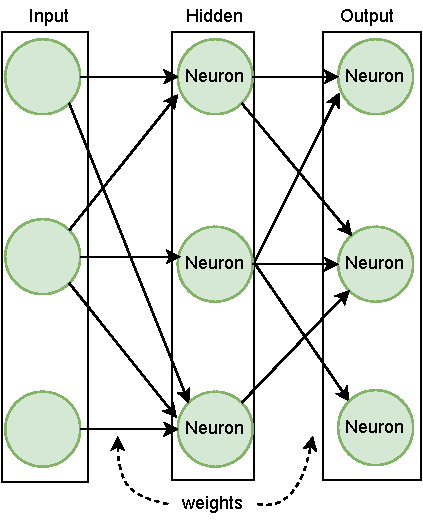
\includegraphics[width=0.2\textwidth]{simpleFFNN}
		\label{fig:simpleNN}}
	\hfil
	\subfloat[]
	{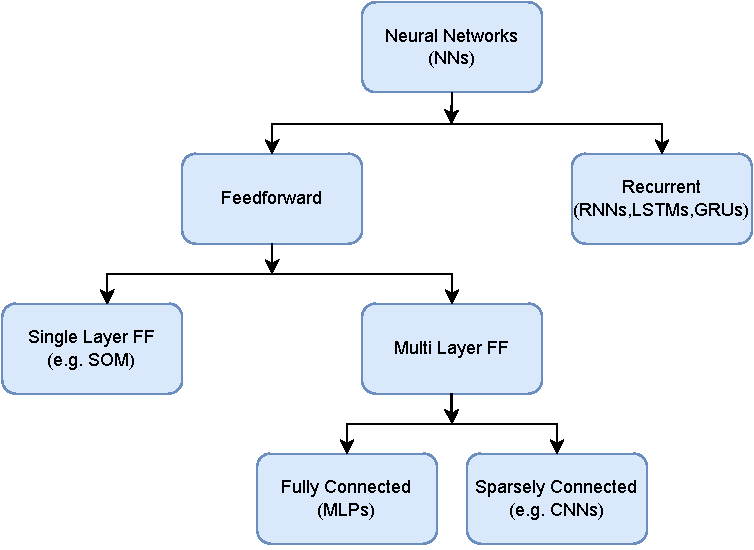
\includegraphics[width=0.5\textwidth]{nnClassification}
		\label{fig:nnClassification}}
	\hfil
	\caption{(a) Example of simple Neural Network. (b) Broad categories of NNs.}
	\label{fig:intro}
\end{figure}
\subsection{Broad Classification}
There are several classes of NNs that differ from each other in the number of neurons, connections between them, and method of training. \figurename{~\ref{fig:nnClassification}} shows two broad classes of NNs, feedforward neural networks (FFNNs) and recurrent neural networks (RNNs). 

FFNNs approximate some function to map input to output using a set of parameters (weights and biases). In FFNNs, the data flows from the input layer to the output layer via intermediate layers a.k.a. hidden layers, and there are no feedback connections. These can be represented as directed acyclic graphs. FFNNs do not have any internal state, and output depends on the current input and the parameters. Based on the number of layers, FFNNs can be further classified as single-layer and multi-layer FFNNs. Single-layer Feedforward NNs consist of just two layers - an input and an output layer. Only the output layer performs computation. Self-Organizing Maps (SOMs) are examples of single-layer NNs and are used in dimensionality reduction and clustering applications. 

Multilayer FFNNs represent the most important class of machine learning algorithms. They are used in several commercial applications and are the stepping stone of several other kind of NNs. They consist of one or more intermediate layers (hidden layers) between the input and output layers. Depending on whether the neurons in the layer are connected to all or a few of the neurons in the previous layers, these can be further classified as fully connected FFNNs (\figurename{~\ref{fig:fullyConnected}}) or sparsely connected FFNNs (\figurename{~\ref{fig:sparselyConnected}}), respectively. One of the most popular class of FFNNs used for image classification and recognition from images is Convolutional Neural Networks (CNNs).

Another popular class of NNs is recurrent neural networks (RNNs), which have layers with loops (\figurename{~\ref{fig:recurrentLayer}}). These loops represent that the output at any step is influenced by the previously seen inputs. These networks extract information from the inputs and store it in an internal state. In this class of NNs, the output depends not only on the current input but also on the internal state. They share the weights across different time steps of the sequence. These networks are widely used in speech recognition, natural language processing (NLP), and other sequential data processing applications. Long short-term memory networks (LSTMs) are among the popular variants of RNNs.

\begin{figure}[!htb]
	\centering
	\captionsetup{font=sf}
	\subfloat[]
	{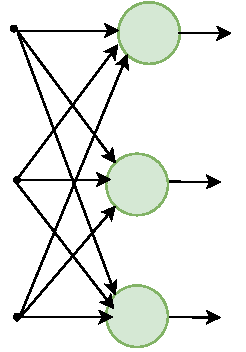
\includegraphics[width=0.15\textwidth]{fullyConnected}
		\label{fig:fullyConnected}}
	\hfil
	\subfloat[]
	{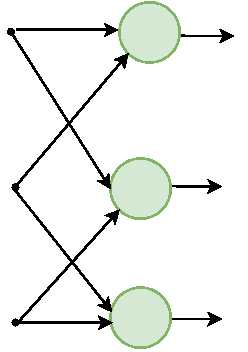
\includegraphics[width=0.15\linewidth]{sparselyConnected}
		\label{fig:sparselyConnected}}
	\hfil
	\subfloat[]
	{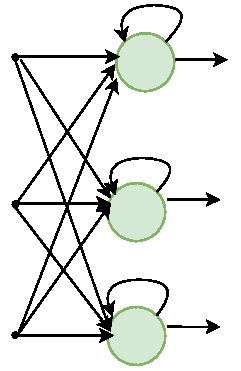
\includegraphics[width=0.15\linewidth]{recurrentLayer}
		\label{fig:recurrentLayer}}
	\caption{Types of NN layers (a) Fully Connected FF. (b) Sparsely Connected FF. (c) Recurrent. }
	\label{fig:nnLayers}
\end{figure}
Multilayer NNs with more than three layers are referred to as deep neural networks (DNNs), capable of learning complex functions. 
\subsection{Training Vs. Inference}
NNs are machine learning algorithms and need not be programmed explicitly. They learn from the raw data to provide solutions to real world problems. For example, to classify the class of an object in an image or to identify the speaker's age, sex from a voice sample. In this learning process they are provided a large set of real world examples and they determine the weights and biases of each neuron. This learning process is referred to as training of the neural network. Once trained the NN can estimate the output for a new set of inputs using the weights and biases learned during the training. Estimating the output for a new input using trained weights and biases is referred to as inference.

The objective of the training is to determine the weights and biases to achieve high accuracy. The accuracy is measured using a score value which estimates the difference between the expected and produced output by the NN. During the training a loss function is used to determine the correctness of the output. Using this loss function, weights are updated using some optimization technique, generally gradient descent. The gradient descent involve computations of partial derivatives to estimate the loss due to each weight by using chain rule of calculas. This involves storing the intermediate output of the network and thus require large storage. During the training, computations are performed using high precision to avoid accuracy loss, which further increases the storage and computations requirements.

Recently, DNN models with several hundreds of layers have been reported~\cite{he2016deep}. These DNNs have millions of parameters (weights and biases). For learning, these DNNs require large training data sets, and need to go through multiple iterations to achieve the desired accuracy, requiring significant computational resources and time. 

\figurename{~\ref{fig:workFlow}} shows difference phases of NNs. The development phase, which is usually performed on desktop/laptop machine. To speed up the development there are several popular NN frameworks e.g., PyTorch, TensorFlow etc. These framework implements layers commonly used in NNs, loss functions, backpropogation etc. They also support  methods to estimate and visualize the accuracy of the NNs, access to freely available training and testing data sets. 
\begin{figure}[!htb]
	\centering
	\captionsetup{font=sf}
	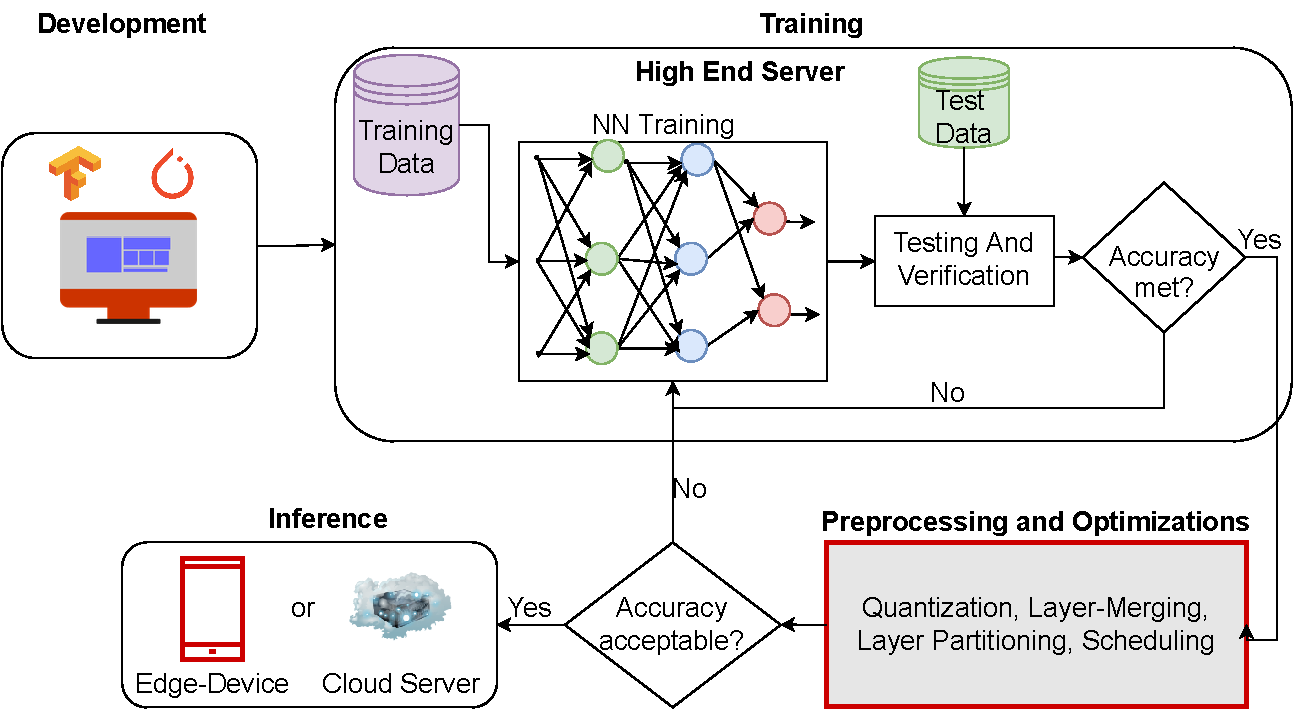
\includegraphics[width=0.7\textwidth]{WorkFlow}
	\caption{Work Flow for Neural Networks.}
	\label{fig:workFlow}
\end{figure}

Training of NNs involve updating weights and biases using large number of input samples. Its a repetitive process, until the desired accuracy is achieved. Training a DNN may last from few hours to several weeks. Hence training of DNNs are generally performed on high performance systems typically using GPUs. NN frameworks provide ways to save the trained model weights and biases which are used in optimization and inference phase. Once these models are trained, they can be deployed in applications for inferencing, where the deployment platforms may range from cloud to embedded devices. 

\begin{figure}[!htb]
	\centering
	\captionsetup{font=sf}
	\subfloat[]
	{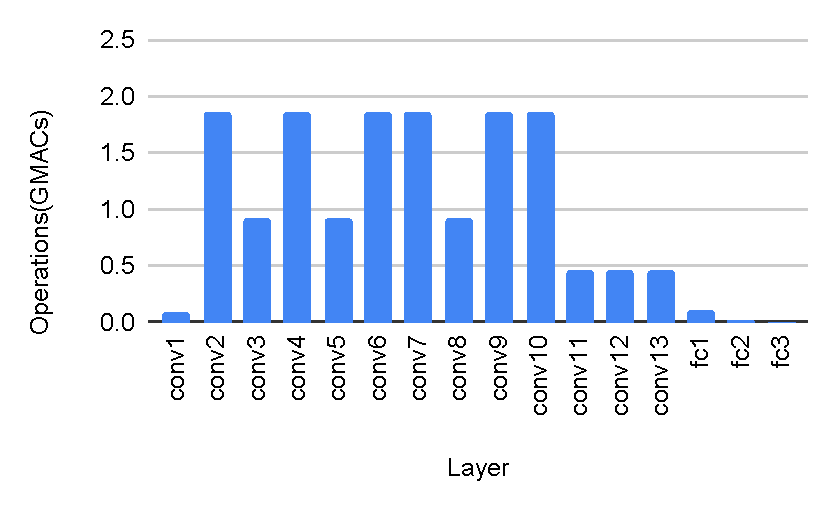
\includegraphics[width=0.45\textwidth]{vgg16GMACsOverview}
		\label{fig:vgg16GMACsOverview}}
	\hfil
	\subfloat[]
	{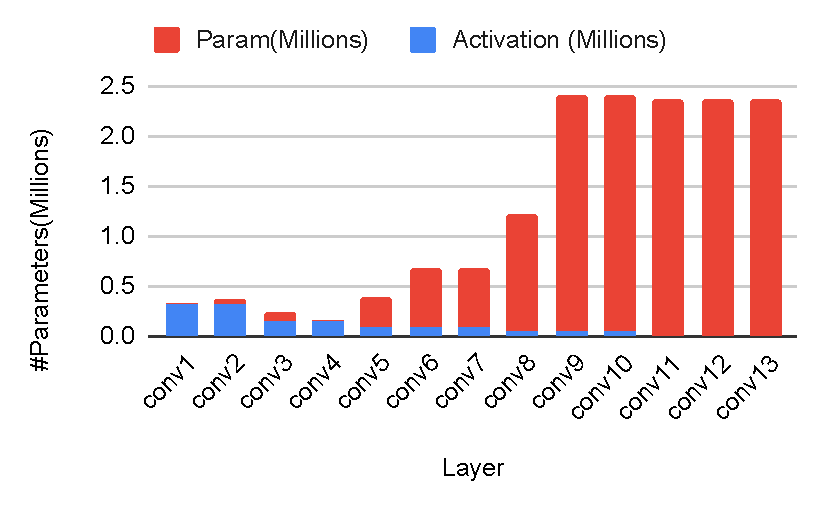
\includegraphics[width=0.45\linewidth]{vgg16ParamsOverview}
		\label{fig:vgg16ParamsOverview}}
	\caption{VGG16: A Convolution NN (a) Multiply And Accumlate Operations (MACs) per Inference. (b) Number of Parameters used per Inference.}
	\label{fig:MACAndParamsSize}
\end{figure}
\figurename{~\ref{fig:vgg16GMACsOverview}} and \figurename{~\ref{fig:vgg16ParamsOverview}} shows the layer wise distribution of number of operations (MACs) and parameters accessed per inference in a popular Convolution NN, VGG16, respectively. Overall for a single inference, VGG16 performs 15.47 GMACs operations and it accesses 138 million parameters. This illustrates, inferencing involve compute and memory intensive operations. If the NNs are deployed on the cloud, the throughput and energy demands are met using high performance systems like GPU. However, if they are deployed on energy and resource constrained edge devices, optimizing these models is a must to meet the targets. In this work we mainly focus on optimizing NN models before they are used for inference in energy constrained edge-devices.

\section{Edge AI}
Few years back, inferencing were commonly performed on the cloud, while the edge devices were used for collecting the real world data. Recent growth of deep learning has enabled several intelligent applications for consumer and edge devices. Today we see explosion of applications using deep learning algorithms in consumer electronic devices like Hello Google, Alexa, Creta. Key enablers of edge AI are deep learning tools, and recent researches in the area of edge AI accelerators. Deep learning tools that were earlier used by researchers to develop the deep learning algorithms, have evolved in past few years and now they can be used by even non-experts to develop intelligent applications for consumer devices like smartphones. Recent research to improve the computation and energy efficiency of Edge AI accelerators also enabled this transition. 

Edge AI is gaining momentum as it improves the user experience, eliminates network bandwidth issues, and improves privacy and security. Due to these reasons, there is a growing trend of shifting the processing of these DNN applications from cloud to edge devices, near the sensors. Manufacturers are shifting the processing of NNs from cloud to edge devices like smartphones and tablets. 

Edge AI devices are battery-operated with limited resources and a tight energy budget which poses significant challenges in processing NNs inference. \figurename{~\ref{fig:edgeAIChallenges}} shows the key challenges for Edge AI devices. Energy efficiency and throughput are the two most important metrics for edge devices. While energy efficiency is of paramount importance for longer battery time, high throughput is desired for better user-response time. Efficient processing of DNNs inferencing on edge devices is critical for their widespread usage. 
\begin{figure}[!htb]
	\centering
	\captionsetup{font=sf}
	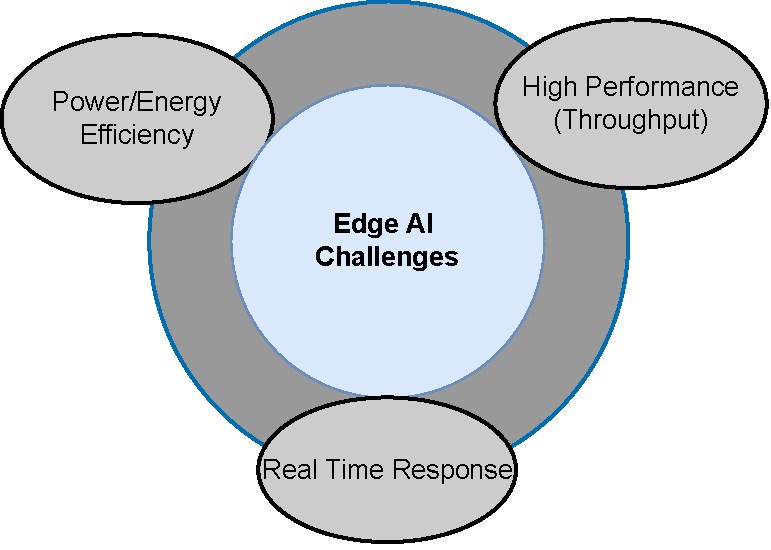
\includegraphics[width=0.6\textwidth]{edgeAIChallenges}
	\caption{Challenges for Edge-AI Accelerator}
	\label{fig:edgeAIChallenges}
\end{figure}
\section{Customized NN Accelerator for Edge Devices}
Edge devices mostly use customized accelerators to meet energy and throughput demands. Several FPGA~\cite{zhang2015optimizing,wei2019overcoming,gokhale2014240,8742284,gupta2015deep,alwani2016fused}, GPU~\cite{chetlur2014cudnn} and ASIC~\cite{Chen2016EyerissAS,chen2014diannao,chen2014dadiannao,du2015shidiannao} accelerators have been proposed to meet the performance and energy targets. 
\begin{figure}[!htb]
	\centering
	\captionsetup{font=sf}
	\subfloat[]
	{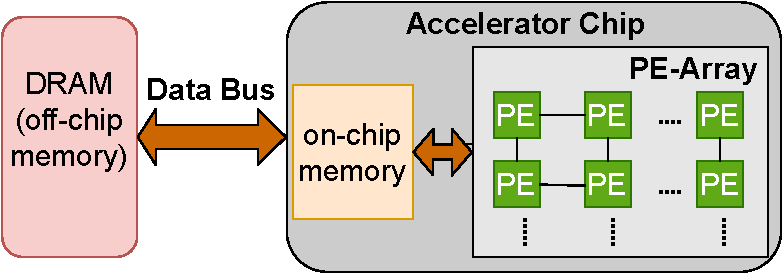
\includegraphics[width=0.45\textwidth]{typicalDNNAccelerator}
		\label{fig:typicalDNNAccelerator}}
	\hfil
	\subfloat[]
	{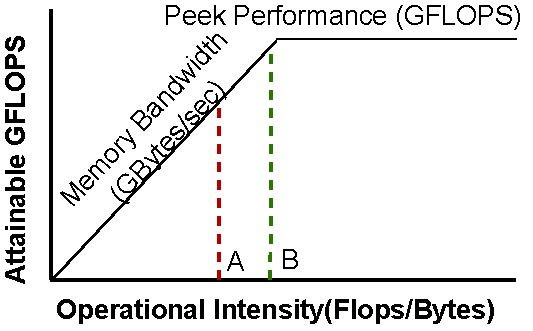
\includegraphics[width=0.4\linewidth]{roofline}
		\label{fig:roofline}}
	\caption{(a) Typical DNN accelerator architecture. (b) Roofline model}
	\label{fig:acceleratorAndRoofline}
\end{figure}
\figurename{~\ref{fig:typicalDNNAccelerator}} shows a typical DNN accelerator architecture, which consists of an off-chip memory and an accelerator chip. An accelerator chip mainly consists of an on-chip memory of a few hundred KBs and an array of Processing Elements (PEs). The accelerator system has multiple memory levels: off-chip memory, on-chip memory, and the registers inside the PEs. Each memory level has different access latency and energy costs. The memory access energy from off-chip memory is up to two orders of magnitude higher than a PE computation operation~\cite{Chen2016EyerissAS}. It has been observed that more than 80\% of the overall energy consumption of these accelerators is due to off-chip memory accesses~\cite{chen2014diannao}. 

The PE-array (\figurename{~\ref{fig:typicalDNNAccelerator}}) has a large number of processing elements, capable of performing several operations per cycle. However, throughput is often limited by off-chip memory bandwidth~\cite{williams2009roofline}. Fig.~\ref{fig:roofline} shows attainable throughput in such a scenario as a function of the operational intensity of an application. The figure shows two application kernels (A and B) with different operational intensities (FLOPS/byte), with performance limited by the memory bandwidth in both cases, which is typically the case for most DNN accelerators. Kernel B, however, has better operational intensity than kernel A and achieves better throughput. Effective data-reuse techniques are required to improve the performance of bandwidth-limited parallel architectures. Therefore, reducing the off-chip memory is the key to improving the throughput and energy efficiency of DNN accelerators. Much recent research has focused on reducing off-chip memory accesses.
\section{Efficient Edge AI Processing}
\begin{figure}[!htb]
	\centering
	\captionsetup{font=sf}
	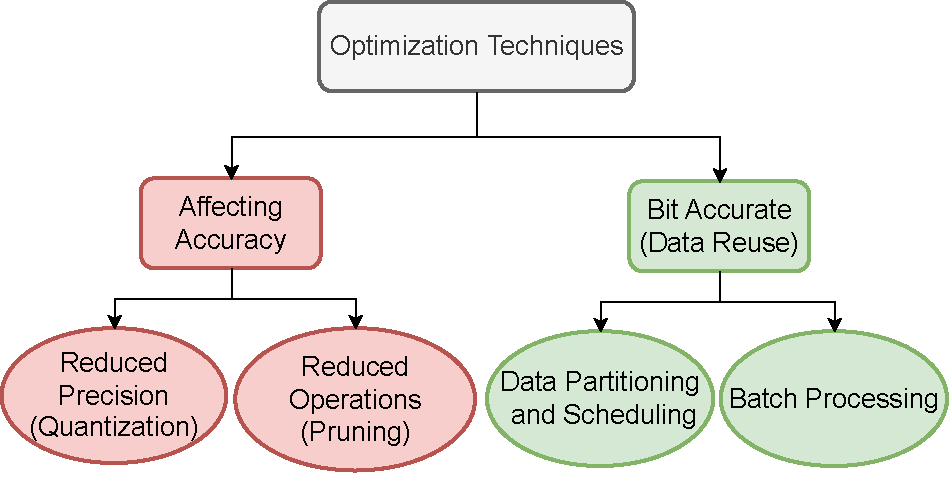
\includegraphics[width=0.5\textwidth]{previousWorkClassification}
	\caption{Broad Classification of previous works for improving the performance of DNN accelerators.}
	\label{fig:previousWorkClassification}
\end{figure}
Recent works that aim to reduce the off-chip memory accesses of NN accelerators can be classified into two broad categories, as shown in Figure~\ref{fig:previousWorkClassification}. One category of work exploits error-tolerance and redundancy in NNs using quantization, compression, and pruning techniques to reduce the precision, the number of operations and models' size~\cite{ferreira2016fpga,wang2018c,chang2015recurrent,han2017ese,lee2016fpga}. With reduced precision, the storage requirement and memory accesses reduce proportionally and improve energy efficiency~\cite{sze2017efficient}. In shallow NNs, the number of parameters is smaller compared to DNNs. Quantization and pruning techniques result in reduced NN model sizes. The reduced model for shallow NNs may fit into the on-chip memory and thus eliminate the off-chip memory bandwidth bottleneck. However, quantization and pruning approaches impact the accuracy of the networks and may not be suitable where accuracy can not be compromised. Also, the number of parameters in modern DNNs is significantly large. For these DNNs, besides quantization and pruning, additional techniques are required to further reduce the off-chip memory accesses.

The other approach, which does not affect the accuracy of the network, is to reduce repeated off-chip accesses to the same NN coefficients when the entire set of NN coefficients does not fit in the on-chip memory. This is quite effective for many modern DNNs (e.g., CNNs, RNNs) with a significantly large number of parameters~\cite{zhang2015optimizing,Li2018SmartShuttleOO,que2019efficient,park2020time}. The weights are repeatedly used for all the inputs during the inference phase. Inputs can be grouped as a batch and processed to reuse the weights. This technique is referred to as batch processing. Increasing the batch size increases the weights reuse but also increases the latency. Another prominent data reuse technique is data partitioning and scheduling. In this technique, the data is partitioned into tiles, and operations on tiles are scheduled in such a way that data can be accessed from the on-chip memory, as far as possible. For a given DNN, there are numerous ways of doing data partitioning and scheduling, offering different extents of data reuse. Choosing an optimal way here is non-trivial.

The data-reuse approaches are orthogonal to the quantization techniques and can be combined to reduce the off-chip memory accesses further. In this work, we have explored both types of approaches and contributed some new ideas.

\section{Summary and Outline of the Thesis} 
Recent advancement in NNs have enabled them to solve several real world problems which long ago was dreamed by the researchers. Due to their high accuracy they are now being used in wide range of domains. Last few years have witnessed the enormous growth in number of intelligent applications targeted for edge devices. However, resource and energy constrained on edge device poses a significant challenge for the wide acceptance of NN applications. Hence there is a pressing need for energy efficient execution of NNs applications. In NN inference phase, large amount of energy consumptions results from expensive off-chip memory accesses. A key to improve the performance and energy efficiency of these edge devices is to optimize the memory accesses.
 
Previous research has shown that for data partitioning and scheduling, making a choice independently for each layer of a NN is better than making a common choice for the entire NN because of the different shapes of various layers. We observe that the choice of optimal data partitioning and scheduling not only depends on the shape of a layer but also on some architectural parameters. We present an analytical framework in Chapter 2 that quantifies the off-chip memory accesses and compute cycles for DNN layers of varying shapes, also taking into account the architectural constraints. It is useful for comparing different data partitioning and scheduling schemes to explore the large design space in order to find the optimal solution for improving the energy and throughput. 

Based on the above analytical framework, in Chapter 3 we propose a data reuse approach that takes into account the architectural parameters and determines the optimal partitioning and scheduling scheme to minimize the off-chip memory access of DNN layers. We demonstrate the efficacy of our partitioning and adaptive scheduling approach on the compute and memory-intensive CNN layers. 

In Chapter 4, we propose a novel data reuse approach to improve the throughput and energy efficiency of state-of-the-art recurrent neural networks (RNNs). The proposed approach splits the computations and combines them in a way that reduces the off-chip memory accesses of large matrices significantly. We measure the design power and memory accesses on FPGA implementation of Long-Short Term Memory Network (LSTM) accelerators and show the energy and throughput improvements achieved by our approach.
	
We analyze the effect of using different bit resolutions on the accuracy of a NN, as well as the benefits of using low bit-width data resolution for self organizing maps (SOMs) for designing energy-constrained systems where the area, power, and performance are of critical importance in Chapter 5. Using an efficient implementation of SOM design on FPGA, which can be configured for different bit resolutions, we show performance comparison for different data precisions. 
	
The work done in this thesis not only improves the state-of-the-art for energy efficient execution of modern NNs, but also gives directions to future research. In chapter 6, we discuss these new research directions together with the conclusion of our work.